%!TEX root = edance.tex


\chapter{AC Circuits and AC Analysis}

\graphicspath{{./figs_AC/}}



%%%%%%%%%%%%%%%%%%%%%%%%%%%%%%%%%%%%%%%%

\subsection{Chapter Preview}

This chapter builds on the previous by focusing solely on AC circuits, or the circuit response in sinusoidal steady state.  We will also focus on circuits in particular and derive an even simpler procedure for analysis based on "phasors", which is just a shorthand way to do the complex exponential response that we discussed in the previous chapter.  We formally introduce the concept of the AC transfer functions in circuits as ratios of signals, either voltage or current, in the frequency domain.  We will see that for circuits of interest, we can completely characterize the transfer function in terms of a finite number of "poles" and "zeros".     We will also discuss the Bode Plot technique for estimating the transfer function and touch briefly on AC power.

 
%%%%%%%%%%%%%%%%%%%%%%%%%%%%%%%%%%%%%%%%
%%%%%%%%%%%%%%%%%%%%%%%%%%%%%%%%%%%%%%%%
%%%%%%%%%%%%%%%%%%%%%%%%%%%%%%%%%%%%%%%%

\section{Transfer Functions}



%%%%%%%%%%%%%%%%%%%%%%%%%%%%%%%%%%%%%%%%
%%%%%%%%%%%%%%%%%%%%%%%%%%%%%%%%%%%%%%%%
%%%%%%%%%%%%%%%%%%%%%%%%%%%%%%%%%%%%%%%%



%%%%%%%%%%%%%%%%%%%%%%%%%%%%%%%%%%%%%%%%

\subsection{Transfer Function Concept}

\begin{figure}[tb]
\begin{center}
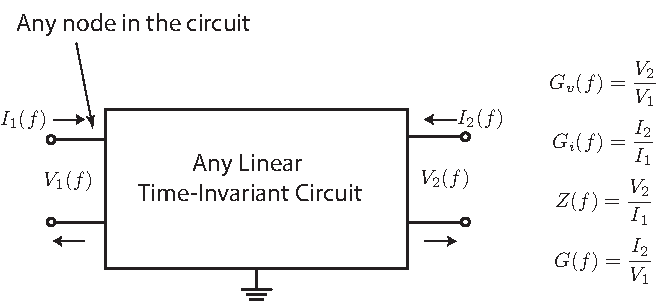
\includegraphics[scale=1]{transfer_func}
\end{center}
\caption{Between two ports in a linear time-invariant (LTI) circuit, we can define four transfer functions.  In this chapter we will focus on the frequency domain transfer functions.} \label{fig:blackboxltiports}
\end{figure}


In many situations, we are interested in the transfer of voltage or current from one terminal pair, or port, to another port in the circuit.  As shown in the blackbox Fig.~\ref{fig:blackboxltiports}, we can identify these ports by explicitly labeling them and clearly identifying the voltages across and the currents into and out of these ports.  Note that some ports may have terminals in common, such as a common-ground for ground referenced signals.  

The key is that we drive a pair of nodes with a sinusoidal current or voltage -- \textit{the input}, and observe the output across a load at another pair of terminals -- \textit{the output}.  The ratio is the transfer function.  For a fixed frequency, it’s just a complex number.  From the last chapter, we know it's the  Laplace transform of the impulse response evaluated on the $j\omega$ axis.
 


%%%%%%%%%%%%%%%%%%%%%%%%%%%%%%%%%%%%%%%%

\subsubsection{Example 1 – ECG Amplifier}

The electrocardiogram (ECG) is a measurement of the voltage between two points on the body.  For example, as shown in Fig.~\ref{fig:ecg}, the voltage across the chest measured from the "right arm" (RA) to the "left arm" (LA) is what's known as lead I.  The ground reference is often the "right leg" (RL).  This voltage is the "input voltage" and we need to amplify it and reject any common-mode noise (see Section~\ref{sec:cmrr}), especially 60 Hz or 50 Hz AC line voltage, which is often orders of magnitude larger than the desired signal.  The output voltage may be single-ended and referenced to a different ground, as shown in the figure. 

In this scenario, we define the transfer function as
\begin{equation}
     G_v(f) = \frac{V_{out}}{V_1 - V_2 }
\end{equation}

The variation in frequency is due to the frequency content of the heartbeat signal and possibly filters applied to the signal intentionally to reduce the impact of noise.

\begin{figure}[tb]
\begin{center}
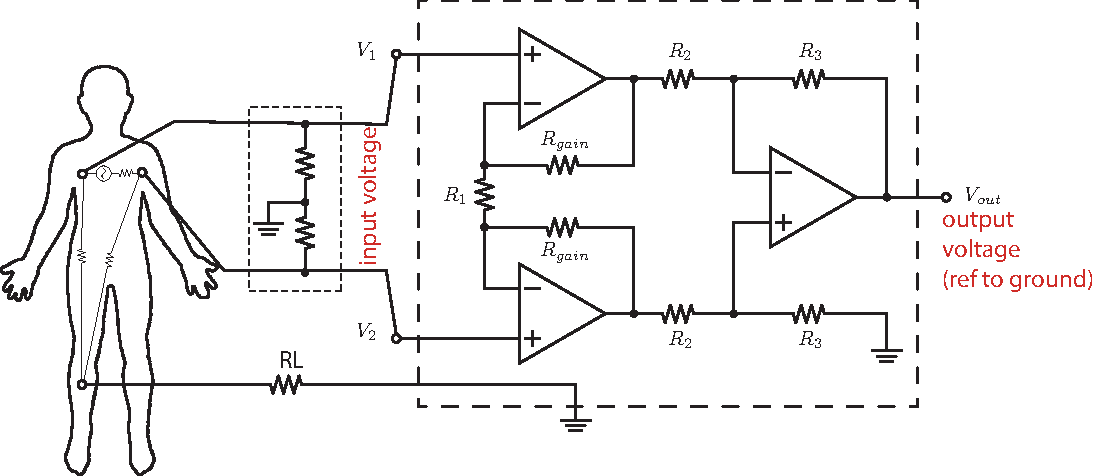
\includegraphics[width=.95\columnwidth]{ex_opamp-ia2}
\end{center}
\caption{An ECG amplifier is an example of a transfer function from a non-ground referenced port to an output port that is referenced to ground, or a differential to single-ended transfer function.} \label{fig:ecg}
\end{figure}



%%%%%%%%%%%%%%%%%%%%%%%%%%%%%%%%%%%%%%%%

\subsubsection{Example 2 – Mic/Speaker}

\begin{figure}[tb]
\begin{center}
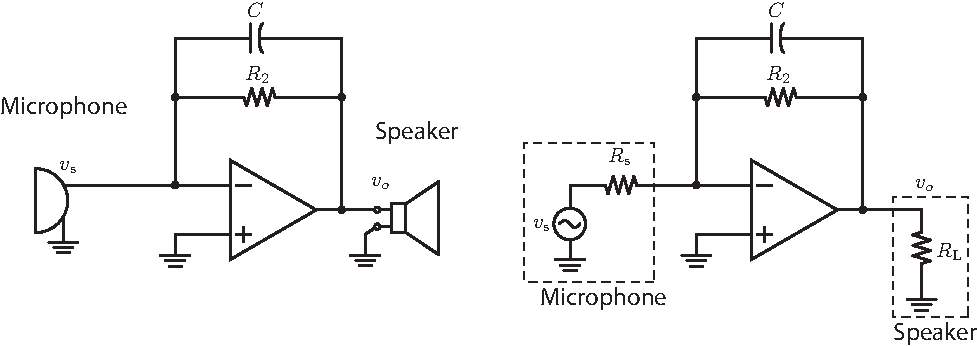
\includegraphics[width=\columnwidth]{ex_microphone}
\end{center}
\caption{The transfer function from a microphone to the output of the amplifier is actually a current to voltage transfer function.  Note the voltage to voltage transfer function is undefined for an ideal op-amp since the negative input terminal is a virtual ground.} \label{fig:microphone}
\end{figure}


The next example is deceptively simple because on first inspection of Fig.~\ref{fig:microphone}a, you may conclude that there's an error in the drawing, because the negative input of the inverting amplifier is shorted due to the "virtual ground" connection.  In fact, were it not for the microphone source resistance, as shown in  Fig.~\ref{fig:microphone}b, this would be the case. But the signal is amplified and filtered by the presence of $C$ in the inverting amplifier configuration.  Low frequency signals see a gain 
\begin{equation}
     G_v(f) = \frac{v_{o}}{v_s }
\end{equation}
of $-R_2/R_s$ whereas very high frequency signals see very small gain because as the capacitor becomes more conductive than the resistor $R_2$, or in other words $\omega C \gg R_2$, then the gain is simply
\begin{equation}
	G_v(f) \sim \frac{-\frac{1}{\omega C}}{R_2 } = \frac{-1}{\omega C R_2 }
\end{equation}
In this example, the presence of the source impedance changed everything.  In general we must be careful to include the potential impact of the source/load impedances.  



%%%%%%%%%%%%%%%%%%%%%%%%%%%%%%%%%%%%%%%%

\subsubsection{Example 3 – Photodetector}

\begin{figure}[tb]
\begin{center}
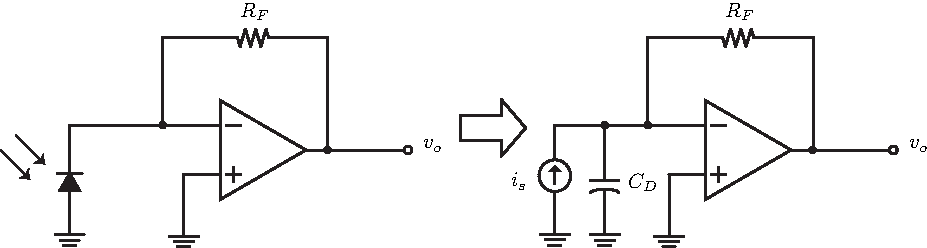
\includegraphics[width=.8\columnwidth]{ex_photodetect}
\end{center}
\caption{A photo-detector is used to convert photons to current, which are then converted into a voltage through the trans-impedance amplifier (TIA).  The figure on the right is the equivalent circuit model.} \label{fig:pd_detect}
\end{figure}


For many applications, we need to process a voltage, so a "transimpednace" amplifier is needed to convert the current to the voltage through $R_F$ as shown.\footnote{Why not simply use a resistor in parallel with the diode to convert the current into a voltage?}

Shown in Fig.~\ref{fig:pd_detect}, the source is a photodiode, a device that has an output current proportional to the number of impinging photons.  Again, upon first inspection it seems that the diode is "shorted" to ground through the virtual ground connection, but the diode is better modeled as a current source.  The input current is therefore the signal of interest, as shown in the same figure.  It's important to include the source capacitance ($C_D$), which limits the high frequency performance.  Once benefit of the amplifier is that the signal across $C_D$ is mostly shorted and therefore the impact is not as severe as it would be otherwise.









%%%%%%%%%%%%%%%%%%%%%%%%%%%%%%%%%%%%%%%%

\subsection{Voltage and Current Gain}

\begin{figure}[tb]
\begin{center}
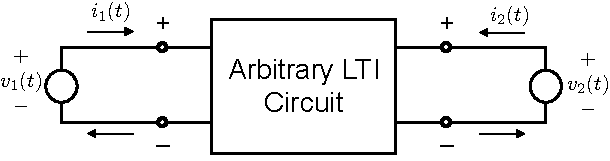
\includegraphics[width=.6\columnwidth]{mod1_3_1_twoport}
\end{center}
\caption{An arbitrary two-port consisting of a linear time-invariant circuit.} \label{fig:twoportivgain}
\end{figure}


The voltage (current) gain is just the voltage (current) transfer function from one port to another port (see Fig.~\ref{fig:twoportivgain}:
\begin{equation}
{G_v}(\omega ) = \frac{{{V_2}}}{{{V_1}}} = \left| {\frac{{{V_2}}}{{{V_1}}}} \right|{e^{j({\varphi _2} - {\varphi _1})}}
\end{equation}
\begin{equation}
{G_i}(\omega ) = \frac{{{I_2}}}{{{I_1}}} = \left| {\frac{{{I_2}}}{{{I_1}}}} \right|{e^{j({\varphi _2} - {\varphi _1})}}
\end{equation}
If \textit{G > }1, the circuit has voltage (current) gain.   If \textit{G} < 1, the circuit has loss or attenuation.   It's a common misconception that only "active" circuits can have gain.  We'll demonstrate in section~\ref{sec:lcr} that $LCR$ circuits in particular are passive and can provide voltage and or current gain.  Another common example is the ubiquitous transformer, which provides gain through mutual coupling.  It may surprise you that even $RC$ circuits can provide gain, although not as easily as with inductors and transformers !
 


%%%%%%%%%%%%%%%%%%%%%%%%%%%%%%%%%%%%%%%%

\subsection{Trans-Impedance and Trans-Admittance}


Current/voltage gain are unitless quantities but we can define a signal as a voltage or a current, or both (or even a power, or the product).   If the transfer involves voltage to current or vice versa, we must be careful to define the units.  We have a trans-impedance (TIA) amplifier gain
\begin{equation}
J(\omega ) = \frac{{{V_2}}}{{{I_1}}} = \left| {\frac{{{V_2}}}{{{I_1}}}} \right|{e^{j({\varphi _2} - {\varphi _1})}}  [\Omega ]
\end{equation}
Less commonly, we have a voltage to current amplifier:
\begin{equation}
K(\omega ) = \frac{{{I_2}}}{{{V_1}}} = \left| {\frac{{{I_2}}}{{{V_1}}}} \right|{e^{j({\varphi _2} - {\varphi _1})}}  [S]
\end{equation}

 
%%%%%%%%%%%%%%%%%%%%%%%%%%%%%%%%%%%%%%%%

\subsection{Impede the Currents !}
 
 
 
 \begin{figure}[tb]
\begin{center}
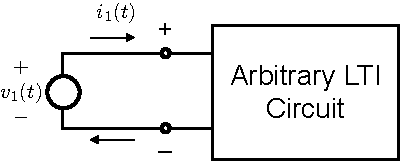
\includegraphics[width=.5\columnwidth]{mod1_3_2_oneport}
\end{center}
\caption{An arbitrary one-port linear time-invariant circuit.} \label{fig:oneport}
\end{figure}

Suppose that the "input" is defined as the voltage of a terminal pair (\textit{port}) and the “output” is defined as the current into the port (see Fig.~\ref{fig:oneport}).  
\begin{equation}
v(t) = V{e^{j\omega t}} = \left| V \right|{e^{j(\omega t + {\varphi _v})}}
\end{equation}
\begin{equation}
i(t) = I{e^{j\omega t}} = \left| I \right|{e^{j(\omega t + {\varphi _i})}}
\end{equation}
The \underline{impedance} $Z$  is defined as the ratio of the phasor voltage to phasor current (“self” transfer function):
\begin{equation}
Z(\omega ) = H(\omega ) = \frac{V}{I} = \left| {\frac{V}{I}} \right|{e^{j({\varphi _v} - {\varphi _i})}}
\end{equation}
We are of course familiar with the concept of impedance $Z$, but even though we may not think about it as a transfer function, it is indeed a transfer function.


\subsection{Admit the Currents!}

Similarly, suppose that the "input" is defined as the current of a terminal pair (\textit{port}) and the “output” is defined as the voltage into the port. The \underline{admmittance} $Y$ is defined as the ratio of the current to voltage (“self” transfer function)
 \begin{equation}
Y(\omega ) = H(\omega ) = \frac{I}{V} = \left| {\frac{I}{V}} \right|{e^{j({\varphi _i} - {\varphi _v})}}
\end{equation}



%%%%%%%%%%%%%%%%%%%%%%%%%%%%%%%%%%%%%%%%
%%%%%%%%%%%%%%%%%%%%%%%%%%%%%%%%%%%%%%%%
%%%%%%%%%%%%%%%%%%%%%%%%%%%%%%%%%%%%%%%%

\section{Transfer Function Poles/Zeros}



%%%%%%%%%%%%%%%%%%%%%%%%%%%%%%%%%%%%%%%%
%%%%%%%%%%%%%%%%%%%%%%%%%%%%%%%%%%%%%%%%
%%%%%%%%%%%%%%%%%%%%%%%%%%%%%%%%%%%%%%%%

%%%%%%%%%%%%%%%%%%%%%%%%%%%%%%%%%%%%%%%%

\subsection{Complex Transfer Function}

Following our derivation from the last chapter, we excite a system with an input voltage (current) \textit{x} and define the output voltage \textit{y} (current) to be any node voltage (branch current).  For a complex exponential input, the "transfer function" from input to output is given by:
\begin{equation}
	H \equiv \frac{y}{x} = \left( {a + {b_1}j\omega  + {b_2}{{(j\omega )}^2} +  \cdots  + \frac{{{c_1}}}{{j\omega }} + \frac{{{c_2}}}{{{{(j\omega )}^2}}} +  \cdots } \right)
\end{equation}
 We can write this in canonical form as a rational function:
\begin{equation}
	H(\omega ) = \frac{{{n_1} + {n_2}j\omega  + {n_3}{{(j\omega )}^2} +  \cdots }}{{{d_1} + {d_2}j\omega  + {d_3}{{(j\omega )}^2} +  \cdots }}
\end{equation}
This form of the equation shows that the numerator and denominator are in general polynomial equations, and polynomial equations are characterized by either their coefficients or more importantly their roots. 

%%%%%%%%%%%%%%%%%%%%%%%%%%%%%%%%%%%%%%%%

\subsubsection{“s” Complex Plane}

You may hear people talking about transfer functions as a function of complex “s” rather than frequency
\begin{equation}
	H(s) = \frac{{({z_1} - s)({z_2} - s) \cdots }}{{({p_1} - s)({p_2} - s) \cdots }}
\end{equation}
As we learned, this is a generalization (Laplace Domain) of frequency. When doing AC analysis, we are deriving the function along the imaginary axis (sinusoidal steady-state response)
\begin{equation}
	H(s = j\omega ) = \frac{{({z_1} - j\omega )({z_2} - j\omega ) \cdots }}{{({p_1} - j\omega )({p_2} - j\omega ) \cdots }}
\end{equation}
This is why you may see introduce this notation:  $H(j\omega )$

 
%%%%%%%%%%%%%%%%%%%%%%%%%%%%%%%%%%%%%%%%

\subsection{Poles and Zeros}

For most circuits that we deal with, the transfer function can be shown to be a rational function
\begin{equation}
	H(\omega ) = \frac{{{n_1} + {n_2}j\omega  + {n_3}{{(j\omega )}^2} +  \cdots }}{{{d_1} + {d_2}j\omega  + {d_3}{{(j\omega )}^2} +  \cdots }}
\end{equation}
The behavior of the circuit can be extracted by finding the roots of the numerator and denominator
\begin{equation} 
	H(\omega ) = \frac{{({z_1} - j\omega )({z_2} - j\omega ) \cdots }}{{({p_1} - j\omega )({p_2} - j\omega ) \cdots }} = \frac{{\prod {({z_i} - j\omega )} }}{{\prod {({p_i} - j\omega )} }}
\end{equation}
Or in another form (DC gain explicit)
\begin{equation}
	H(\omega ) = {G_0}{(j\omega )^K}\frac{{(1 - j\omega {\tau _{z1}})(1 - j\omega {\tau _{z2}}) \cdots }}{{(1 - j\omega {\tau _{p2}})(1 - j\omega {\tau _{p2}}) \cdots }}
\end{equation}	
\begin{equation} = {G_0}{(j\omega )^K}\frac{{\prod {(1 - j\omega {\tau _{z,i}})} }}{{\prod {(1 - j\omega {\tau _{p,i}})} }}
\end{equation}


\subsubsection{Building Tents: Poles and Zeros}

The roots of the numerator are called the “zeros” since at these frequencies, the transfer function is zero.  These are the "stakes in the ground" of our tent, see Fig.~\ref{fig:tent}.  	The roots of the denominator are called the “poles”, since at these frequencies the transfer function peaks (like a pole in a tent).
	 
\begin{figure}[tb]
\begin{center}
\includegraphics[angle=-0.0,width=.8\columnwidth]{image_11.jpg}
\end{center}
\caption{A tent has poles and "zeros", or locations of stakes.  At the stakes the elevation is at ground (zero), whereas at the poles the elevation hits a local maximum. } \label{fig:tent}
\end{figure}

While the frequency response requires us to keep track of the transfer function over a continuous frequency spectrum, this perspective gives us a new insight.  We actually can completely characterize a system by a finite number of poles and zeros.  Come to think of it, this should be obvious because our circuit is built out of a finite number of components ($L$, $C$, $M$, and dependent sources).  So the number of poles and zeros should be related to the number of elements with "memory", such as inductors and capacitors.  


%%%%%%%%%%%%%%%%%%%%%%%%%%%%%%%%%%%%%%%%
%%%%%%%%%%%%%%%%%%%%%%%%%%%%%%%%%%%%%%%%
%%%%%%%%%%%%%%%%%%%%%%%%%%%%%%%%%%%%%%%%

\section{AC Circuits Review}



%%%%%%%%%%%%%%%%%%%%%%%%%%%%%%%%%%%%%%%%
%%%%%%%%%%%%%%%%%%%%%%%%%%%%%%%%%%%%%%%%
%%%%%%%%%%%%%%%%%%%%%%%%%%%%%%%%%%%%%%%%


%%%%%%%%%%%%%%%%%%%%%%%%%%%%%%%%%%%%%%%%

\subsection{Phasors}



  
With our new confidence in complex numbers, we can go full steam ahead and work directly with them … we can even drop the time factor $e^{j\omega t}$ since it will cancel out of the equations.  In other words, the part that matters is the amplitude and phase shift of the resulting complex exponential, not the complex exponential itself.  Let's define this part as the "phasor".

We excite system with a phasor: ${\tilde V_1} = {V_1}{e^{j{\varphi _1}}}$ and the response  will also be phasor: ${\tilde V_2} = {V_2}{e^{j{\varphi _2}}}$.   
 
 

%%%%%%%%%%%%%%%%%%%%%%%%%%%%%%%%%%%%%%%%

\subsection{Capacitor I-V Phasor Relation}

  
To find the phasor relation for current and voltage for a capacitor, begin with the "$I-V$" relation in the time domain (see Fig.~\ref{fig:lcphasor})
 \begin{equation}
{ i_c}(t) = C\frac{{d{v_C}(t)}}{{dt}}
 \end{equation}
Now for sinusoidal steady state we substitute
\begin{equation}
{i_c}(t) = {I_c}{e^{j\omega t}}\\
\end{equation}
and
\begin{equation}
{v_c}(t) = {V_c}{e^{j\omega t}}
\end{equation}
This leads to
\begin{equation}
{I_c}{e^{j\omega t}} = C\frac{d}{{dt}}[{V_c}{e^{j\omega t}}]
\end{equation}
or
\begin{equation}
C{V_c}\frac{d}{{dt}}{e^{j\omega t}} = j\omega \,C{V_c}{e^{j\omega t}}
\end{equation}
Let's eliminate the common $e^{j\omega t}$ factor
\begin{equation}
{I_c}{e^{j\omega t}} = j\omega \,C{V_c}{e^{j\omega t}}
\end{equation}
Or more simply, the phasor relation.  
\begin{equation}
{I_c} = j\omega \,C\,{V_c}
\end{equation}
This is "Ohm's Law" in the frequency domain for a capacitor.

\begin{figure}[tb]
\begin{center}
\begin{tabular}{ccc}
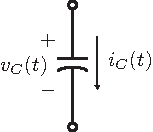
\includegraphics[width=.25\columnwidth]{mod1_3_3_cap} & \hspace{1cm} &
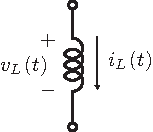
\includegraphics[width=.25\columnwidth]{mod1_3_4_ind} \\
(a) & & (b) \\
\end{tabular}
\end{center}
\caption{(a) Capacitor and (b) inductor  $I$-$V$ relations in the time domain. } \label{fig:lcphasor}
\end{figure}


%%%%%%%%%%%%%%%%%%%%%%%%%%%%%%%%%%%%%%%%

\subsection{Inductor I-V Phasor Relation}

Let's now find the phasor relation for current and voltage in an inductor using the same procedure:
\begin{equation}
v(t) = L\frac{{di(t)}}{{dt}}
\end{equation} 
For sinusoidal steady-state, this implies
\begin{equation}
V{e^{j\omega t}} = L\frac{d}{{dt}}[I{e^{j\omega t}}]
\end{equation}
or
\begin{equation}
LI\frac{d}{{dt}}{e^{j\omega t}} = j\omega \,LI{e^{j\omega t}}
\end{equation}
Canceling the common factor
\begin{equation}
V{e^{j\omega t}} = j\omega \,LI{e^{j\omega t}}
\end{equation}
This is the phasor relation for an inductor, or "Ohm's Law" in the frequency domain for an inductor:
\begin{equation}
V = j\omega \,L\,I
\end{equation}




%%%%%%%%%%%%%%%%%%%%%%%%%%%%%%%%%%%%%%%%

\subsection{Direct Calculation of \textit{H} (no DEs)}

To directly calculate the transfer function (impedance, trans-impedance, etc) we can generalize the circuit analysis concept from the “real” domain to the “phasor” domain.   We drop the time dependence $e^{j\omega t}$ (common factor that cancels out) and just keep track of amplitude and phase (phasor).  With the concept of impedance (admittance), we directly analyze a circuit without explicitly writing down any differential equations.  We are free to use KVL, KCL, mesh analysis, loop analysis, or nodal analysis where inductors and capacitors are treated as complex resistors, or more correctly as an impedance (or admittance).


%%%%%%%%%%%%%%%%%%%%%%%%%%%%%%%%%%%%%%%%
%%%%%%%%%%%%%%%%%%%%%%%%%%%%%%%%%%%%%%%%
%%%%%%%%%%%%%%%%%%%%%%%%%%%%%%%%%%%%%%%%

\section{Example AC Circuit Problems}





%%%%%%%%%%%%%%%%%%%%%%%%%%%%%%%%%%%%%%%%

\subsection{LPF Example: Again!}

In Fig.~\ref{fig:lpfagain}, we show a "real"  time-domain circuit and the corresponding frequency-domain “phasor” circuit.   Instead of setting up the DE in the time-domain, we prefer to do calculations directly in the frequency domain using phasors, treating the capacitor as an imaginary "resistance" or impedance.     We know the impedances: ${Z_R} = R $ and $ {Z_C} = \frac{1}{{j\omega C}}$.



\begin{figure}[tb]
\begin{center}
\begin{tabular}{cc}
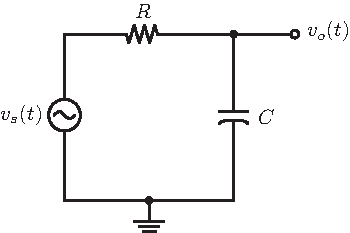
\includegraphics[angle=-0.0,scale=1]{mod1_3_5_rc_lpf} &
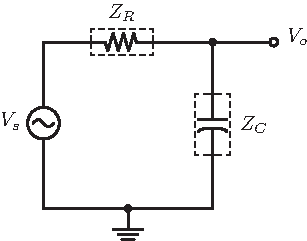
\includegraphics[angle=-0.0,scale=1]{mod1_3_6_rc_lpf_Z} \\
(a) & (b) \\
\end{tabular}
\end{center}
\caption{(a) The low-pass filter in the time domain and (b) an AC equivalent circuit.} \label{fig:lpfagain}
\end{figure}


The fastest way to solve the problem is to say that the LPF is really a voltage divider:
\begin{equation}
H(\omega ) = \frac{{{V_o}}}{{{V_s}}} = \frac{{{Z_C}}}{{{Z_C} + {Z_R}}} = \frac{{\frac{1}{{j\omega C}}}}{{R + \frac{1}{{j\omega C}}}} = \frac{1}{{1 + j\omega RC}}
\end{equation}



%%%%%%%%%%%%%%%%%%%%%%%%%%%%%%%%%%%%%%%%

\subsection{Bigger Example (no problem!)}

\begin{figure}[tb]
\begin{center}
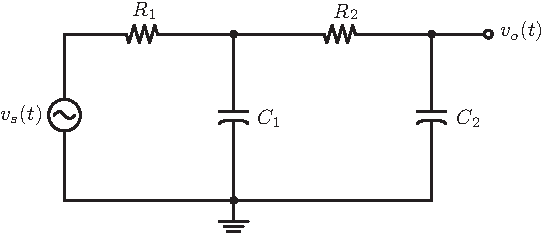
\includegraphics[angle=-0.0,scale=1]{mod1_3_7_rc_lpf2}
\end{center}
\caption{A circuit with two resistors and two capacitors can be analyzed quickly using nodal analysis or circuit theorems by treating the capacitors as impedances.} \label{fig:bigexample}
\end{figure}


  
Consider a more complicated example shown in Fig.~\ref{fig:bigexample}.  To find $v_o$, you can do nodal analysis or use network theorems to simplify the circuit.  Let's find the Thevenin equivalent from $C_2$'s perspective.  The open-circuit voltage is just the first voltage divider:
\begin{equation}
	v_{th} = \frac{Z_{C_1}}{R_1 + Z_{C_1}} v_s 
\end{equation}
The impedance looking into the circuit from $C_2$ is given by
\begin{equation}
	Z_{th} = R_2 + R_1 || Z_{C_1}
\end{equation}
Therefore we have  
\begin{equation}
	v_o = \frac{Z_{C_2}}{Z_{C_2} + Z_{th}} V_{th} 
\end{equation}


%%%%%%%%%%%%%%%%%%%%%%%%%%%%%%%%%%%%%%%%%%%%%%%%%%%%%%%%%%%%%%%%%%%%%%%%%%

\subsection{Series RLC Circuits} \label{sec:lcr}

\begin{figure}
\begin{center}
\includegraphics[scale=1]{rlc}
\end{center}
\caption{A series $RLC$ circuit. } \label{fig:rlc}
\end{figure}

The $RLC$ circuit shown in Fig.~\ref{fig:rlc} is simple but extremely useful and rich in application.  The impedance seen by the source is simply given by
\begin{equation}
  Z = j\omega L + \frac{1}{j\omega C} + R 
    = R + j\omega L \left( 1 - \frac{1}{\omega^2 LC}\right) 
\end{equation}
The impedance is purely real at at the \emph{resonant frequency}, or
when $\Im(Z) = 0$, which happens at a frequency $\omega = \pm \frac{1}{\sqrt{L C}}$.  At resonance the impedance takes on a minimal value.  


\subsubsection{Series Resonance}

\begin{figure}
\begin{center}
\includegraphics[scale=.8]{rlcphasor}
\end{center}
\caption{The phasor diagram shows the relations between the voltages across each component.  Note that the inductor/capacitor voltages are exactly $180^\circ$ degrees out of phase.  Below resonance, the reactance of the capacitor domiants, whereas above resonance, the reactance of the inductor dominates.  At resonance, these reactances are equal and so the voltages across the circuit sum to $v_R$, so the entire source voltage is appleid to the resistor $R$. } \label{fig:rlcphasor}
\end{figure}

It's worthwhile to investigate the cause of resonance, or the cancellation of the reactive
components due to the inductor and capacitor.  Since the inductor and
capacitor voltages are always $180^\circ$ out of phase, and one reactance is dropping while the other is increasing, there is clearly always a frequency when the magnitudes
are equal.    Resonance occurs when $\omega L = \frac{1}{\omega C}$.  


%%%%%%%%%%%%%%%%%%%%%%%%%%%%%%%%%%%%%%%%%%%%%%%%%%%%%%%%%%%%%%%%%%%%%%%%%%

\subsubsection{Quality Factor}

So what's the magic about this circuit?  The first observation is that at
resonance, the voltage across the reactances can be larger, in fact much
larger, than the voltage across the resistors $R$.  In other words, this
circuit has voltage gain.  Of course it does not have power gain, for it is a
passive circuit after all.  The voltage across the inductor is given by 
\begin{equation}
  v_L = j\omega_0 L i = j\omega_0 L \frac{v_s}{Z(j\omega_0)} = 
        j\omega_0 L \frac{v_s}{R} = j Q \times v_s
\end{equation}
%
 where we have defined a circuit $Q$ factor at resonance as
%
\begin{equation}
   Q = \frac{\omega_0 L}{R}
\end{equation}


\subsubsection{Voltage Multiplication}
%
 It's easy to show that the same voltage multiplication occurs across the
capacitor (the reactances are equal at resonance after all)
%
\begin{equation}
  v_C = \frac{1}{j\omega_0 C} i = \frac{1}{j\omega_0 C}
  \frac{v_s}{Z(j\omega_0)} = \frac{1}{j\omega_0 R C} \frac{v_s}{R} = - j Q
  \times v_s
\end{equation}
%
This voltage multiplication property is the key feature of the
circuit that allows it to be used as an impedance transformer.\footnote{It's important to distinguish this $Q$ factor from the intrinsic $Q$ of the inductor and capacitor.  For now, we assume the inductor  and capacitor are ideal.}



%%%%%%%%%%%%%%%%%%%%%%%%%%%%%%%%%%%%%%%%%%%%%%%%%%%%%%%%%%%%%%%%%%%%%%%%%%

\subsubsection{More of Q}

We can re-write the $Q$ factor in several equivalent forms owing to
the equality of the reactances at resonance
%
\begin{equation} \label{eq:qdefs}
  Q = \frac{\omega_0 L}{R} = 
      \frac{1}{\omega_0 C} \frac{1}{R} = \frac{\sqrt{LC}}{C} \frac{1}{R} =
  \sqrt{\frac{L}{C}} \frac{1}{R} = \frac{Z_0}{R}
\end{equation}
%
where we have defined the $Z_0 = \sqrt{\tfrac{L}{C}}$ as the characteristic
impedance of the circuit.



%%%%%%%%%%%%%%%%%%%%%%%%%%%%%%%%%%%%%%%%%%%%%%%%%%%%%%%%%%%%%%%%%%%%%%%%%%

\subsubsection{Resonant Circuit Transfer Function}

Let's now examine the transfer function of the circuit
\begin{equation}
    H(j\omega) = \frac{v_o}{v_s} = \frac{R}{j\omega L + \frac{1}{j\omega C} +
      R}
\end{equation}
\begin{equation}
    H(j\omega) = \frac{j\omega R C }{1 - \omega^2 LC + j\omega R C}
\end{equation}
 Obviously, the circuit cannot conduct DC current, so there is a
  zero in the transfer function.  The denominator is a quadratic
  polynomial.  It's worthwhile to put it into a standard form that
  quickly reveals important circuit parameters
\begin{equation}
    H(j\omega) = \frac{j\omega \frac{R}{L} }{\frac{1}{LC} +  (j\omega)^2 +
      j\omega \frac{R}{L}}
\end{equation}

Using the definition of $Q$ and $\omega_0$ for the circuit
%
\begin{equation}
    H(j\omega) = \frac{j\omega \frac{\omega_0}{Q} }{\omega_0^2 +  (j\omega)^2 +
      j \frac{\omega\omega_0}{Q}}
\end{equation}
%
 Factoring the denominator with the assumption that $Q > \oh$ gives us the
complex poles of the circuit
%
\begin{equation}
    s^\pm = -\frac{\omega_0}{2 Q} \pm j\omega_0 \sqrt{1 - \frac{1}{4Q^2}}
\end{equation}
%
 The poles have a constant magnitude equal to the resonant frequency
\begin{equation}
    |s| = \sqrt{
    \cancel{\frac{\omega_0^2}{4 Q^2}} 
      + \omega_0^2 \left(1 -
      \cancel{\frac{1}{4Q^2}}
          \right)} = \omega_0
\end{equation}



%%%%%%%%%%%%%%%%%%%%%%%%%%%%%%%%%%%%%%%%%%%%%%%%%%%%%%%%%%%%%%%%%%%%%%%%%%

\subsubsection{Circuit Bandwidth and Selectivity}

\begin{figure}
\begin{center}
\includegraphics[width=.65\columnwidth]{transferrlc}
\end{center}
\caption{The transfer function from source to the resistor voltage as a function of frequency.  Dpending on the component values (circuit $Q$), the transfer function exhibits either low or high selectivity. } \label{fig:transferrlc}
\end{figure}

As we plot the magnitude of the
transfer function (Fig.~\ref{fig:transferrlc}), we see that the selectivity of the circuit is also related inversely to the $Q$ factor.  

 In the limit that $Q \rightarrow \infty$, the
circuit is infinitely selective and only allows signals at resonance
$\omega_0$ to travel to the load.  
 Note that the peak gain in the circuit is
always unity, regardless of $Q$, since at resonance the $L$ and $C$ together
disappear and effectively all the source voltage appears across the load.
 The selectivity of the circuit lends itself well to filter
  applications.  To characterize the peakiness, let's compute the
  frequency when the magnitude squared of the transfer function drops
  by half
\begin{equation}
    | H(j\omega)|^2 = \frac{ \left(\omega \frac{\omega_0}{Q} \right)^2}
                      {\left( \omega_0^2 - \omega^2\right)^2 + 
                       \left( \omega \frac{\omega_0}{Q}\right)^2} =
		      \frac{1}{2}
\end{equation}
This happens when 
%
\begin{equation}
     \left( \frac{\omega_0^2 - \omega^2}{\omega_0\omega / Q}\right)^2 = 1
\end{equation}
%
 Solving the above equation yields four
solutions, corresponding to two positive and two negative frequencies.  The
peakiness is characterized by the difference between these frequencies, or the
bandwidth, given by
%
\begin{equation} \label{eq:3db}
     \Delta\omega = \omega_+ - \omega_- = \frac{\omega_0}{Q}
\end{equation}
%




 The normalized bandwidth is inversely proportional to
the circuit $Q$.
\begin{equation}
     \frac{\Delta\omega}{\omega_0} =\frac{1}{Q}
\end{equation}
%
 You can also show that the resonance frequency is the geometric
  mean frequency of the $3$~dB frequencies


%
\begin{equation}
     \omega_0 = \sqrt{\omega_+ \omega_-}
\end{equation}





%%%%%%%%%%%%%%%%%%%%%%%%%%%%%%%%%%%%%%%%
%%%%%%%%%%%%%%%%%%%%%%%%%%%%%%%%%%%%%%%%
%%%%%%%%%%%%%%%%%%%%%%%%%%%%%%%%%%%%%%%%

\section{Bode Plots}



%%%%%%%%%%%%%%%%%%%%%%%%%%%%%%%%%%%%%%%%
%%%%%%%%%%%%%%%%%%%%%%%%%%%%%%%%%%%%%%%%
%%%%%%%%%%%%%%%%%%%%%%%%%%%%%%%%%%%%%%%%




%%%%%%%%%%%%%%%%%%%%%%%%%%%%%%%%%%%%%%%%

\subsection{Finding the Magnitude and Phase (Quickly!)}

The magnitude of the response can be calculated quickly by using the property of the mag operator:
\begin{equation}
	\left| {H(\omega )} \right| = 
		\left| {{G_0}{{(j\omega )}^K}
			\frac{{(1 - j\omega {\tau _{z1}})(1 - j\omega {\tau _{z2}}) \cdots }}
				{{(1 - j\omega {\tau _{p2}})(1 - j\omega {\tau _{p2}}) \cdots }}} \right|
\end{equation}
Separating out the terms
\begin{equation}
		   = \left| {{G_0}} \right|{\omega ^K}
		 	\frac{{\left| {1 - j\omega {\tau _{z1}}} \right|\left| {1 - j\omega {\tau _{z2}}} \right| \cdots }}
				{{\left| {1 - j\omega {\tau _{p2}}} \right|\left| {1 - j\omega {\tau _{p2}}} \right| \cdots }}
\end{equation}
%
The magnitude at DC depends on $G_0$  and the number of poles/zeros at DC. If $K > 0$,  the DC gain is zero. If $K < 0$, DC gain is infinite. Otherwise if $K = 0$, then DC gain is simply $G_0$.
 
The phase can be computed quickly with the following formula:
%
\begin{equation}
 \angle H(\omega ) =  \angle {G_0}{(j\omega )^K}\frac{{(1 - j\omega {\tau _{z1}})(1 - j\omega {\tau _{z2}}) \cdots }}{{(1 - j\omega {\tau _{p2}})(1 - j\omega {\tau _{p2}}) \cdots }}
\end{equation}
Using the properties of the phase operator:
\begin{equation}
   =  \angle {G_0} +  \angle {(j\omega )^K} +  \angle (1 - j\omega {\tau _{z1}}) +  \angle (1 - j\omega {\tau _{z2}}) +  \cdots 
   -  \angle (1 - j\omega {\tau _{p1}}) -  \angle (1 - j\omega {\tau _{p2}}) -  \cdots 
\end{equation}
Note that the second term is simple to calculate for positive frequencies:
\begin{equation}
 \angle {(j\omega )^K} = K\frac{\pi }{2}
\end{equation}
%
Interpret this as saying that multiplication by \textit{j} is equivalent to rotation by 90 degrees


%%%%%%%%%%%%%%%%%%%%%%%%%%%%%%%%%%%%%%%%

\subsection{Bode Plots}

%\begin{figure}[tb]
%\begin{center}
%\includegraphics[angle=-0.0,width=.75\columnwidth]{dB3}
%\end{center}
%\caption{x} \label{fig:x}
%\end{figure}

A Bode Plot is simply a ``sketch" of the $\log$-$\log$ plot of the magnitude and phase response of a circuit (impedance, transimpedance, gain, …).  It provides insight into the behavior of a circuit as a function of frequency without detailed calculations.  The$\log$ expands the scale so that breakpoints in the transfer function are clearly delineated.  In feedback circuit design, Bode plots are used to “compensate” circuits for stability.
 


%%%%%%%%%%%%%%%%%%%%%%%%%%%%%%%%%%%%%%%%

\subsubsection{Example: High-Pass Filter Bode Plot}

\begin{figure}[tb]
\begin{center}
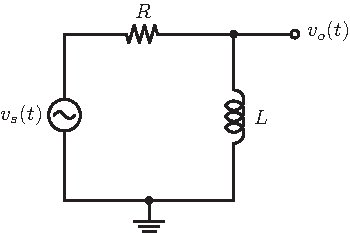
\includegraphics[angle=-0.0,width=.4\columnwidth]{mod1_3_8_rl_hpf}
\end{center}
\caption{A simple $RL$ high-pass filter.} \label{fig:hpf}
\end{figure}

The high-pass filter shown in Fig.~\ref{fig:hpf}  is easily analyzed using a voltage divider:
 \begin{equation}
H(j\omega ) = \frac{{j\omega L}}{{R + j\omega L}} = \frac{{j\omega \frac{L}{R}}}{{1 + j\omega \frac{L}{R}}}\\
  \end{equation}
In terms of normalized time constants:  
\begin{equation}
  H(\omega ) = \frac{{j\omega \tau }}{{1 + j\omega \tau }}
\end{equation}
It's always useful to sanity check your intuition versus equations you derive.  For example, for this circuit we expect (and confirm) the following behavior at various frequencies.  At very high frequencies, the signal must pass through as the inductor is an open circuit:
\begin{equation}
\omega  \to \infty  \quad\quad  \left| H \right| \to \left| {\frac{{j\omega \tau }}{{j\omega \tau }}} \right| = 1
\end{equation}
At DC the output is shorted to ground by the inductor:
\begin{equation}
\omega  \to 0  \quad\quad \left| H \right| \to \frac{0}{{1 + 0}} = 0
\end{equation}
At the breakpoint, the inductance provided the same impedance as the resistor, but the voltage is not half due to the phase difference:
\begin{equation}
\omega  = \frac{1}{\tau }  \quad\quad  \left| H \right| = \left| {\frac{j}{{1 + j}}} \right| = \frac{1}{{\sqrt 2 }}
\end{equation}


%%%%%%%%%%%%%%%%%%%%%%%%%%%%%%%%%%%%%%%%

\subsubsection{HPF Magnitude Bode Plot: Numerator}

Recall that $\log$ of a product is the sum of $\log$s.  So we have
%
\begin{equation}
{\left| {H(\omega )} \right|_{dB}} = {\left| {\frac{{j\omega \tau }}{{1 + j\omega \tau }}} \right|_{dB}} = {\left| {j\omega \tau } \right|_{dB}} + {\left| {\frac{1}{{1 + j\omega \tau }}} \right|_{dB}}
\end{equation}
%
Let's focus on the numerator first.  For this term, $\left|j\omega \tau  \right|_{dB} $, is a straight line and it increases by 20 dB/decade.  This term crosses the 0-dB point at the ``breakpoint", or $\omega = 1/\tau$, as shown in Fig.~\ref{fig:hpfnumden}a:
\begin{equation}
\omega \tau  = 1 \Rightarrow {\left| {j\omega \tau } \right|_{dB}} = 0\,{\rm{dB}}
\end{equation}

\begin{figure}[tb]
\begin{center}
\begin{tabular}{cc}
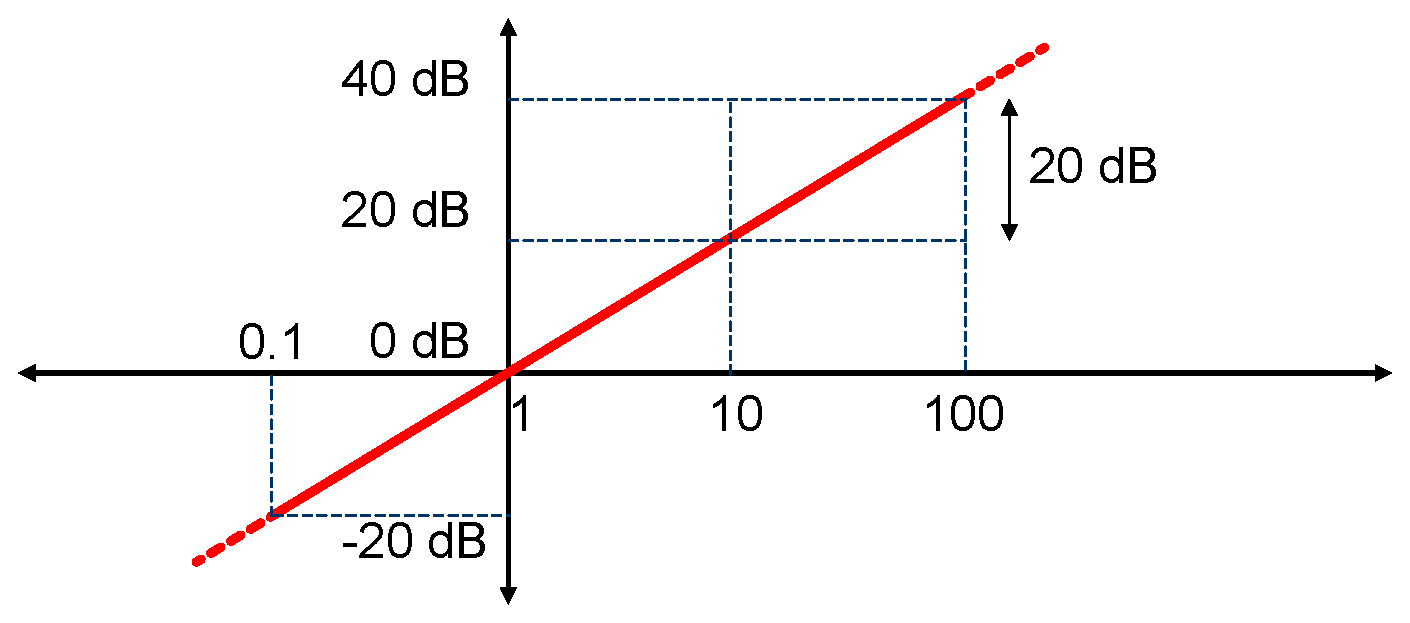
\includegraphics[width=.6\columnwidth]{mod1_3_9_bode1} &
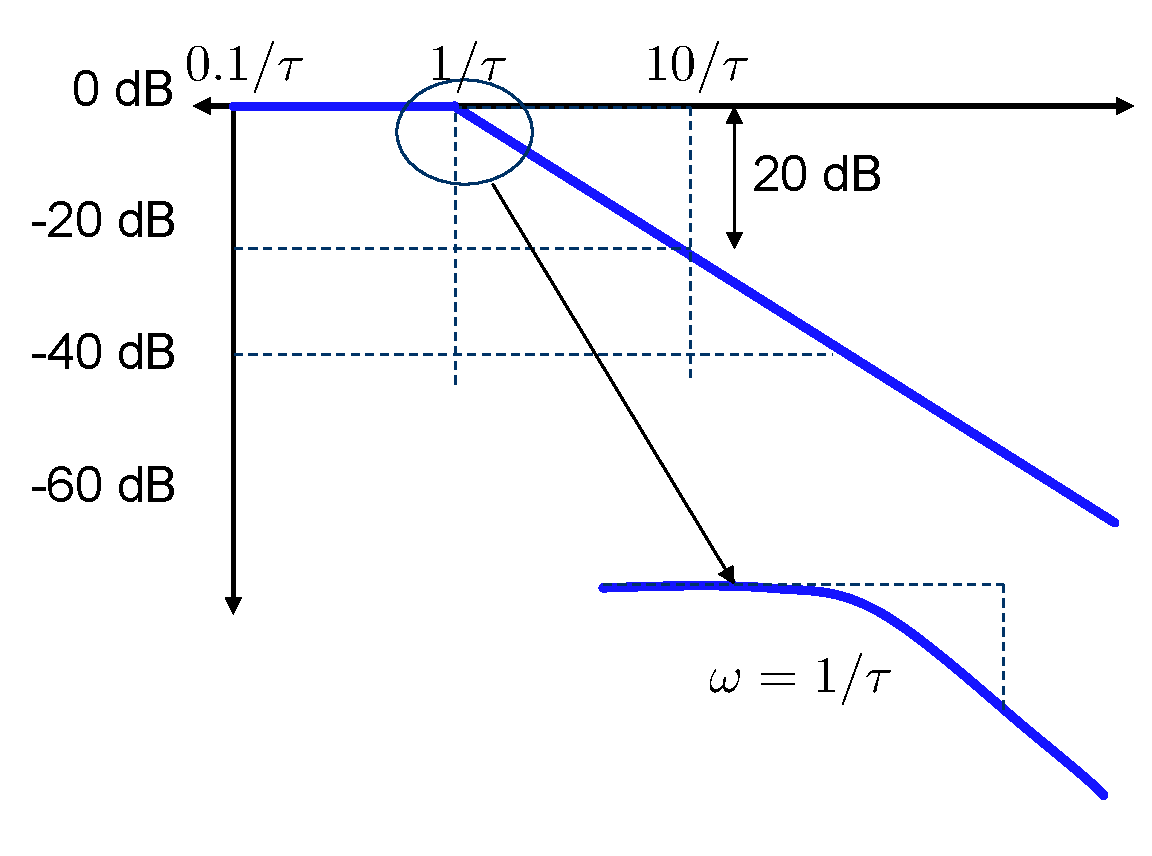
\includegraphics[width=.4\columnwidth]{mod1_3_10_bode2} \\
(a) & (b) \\
\end{tabular}
\end{center}
\caption{Sketch of the magnitude response for (a) $j\omega \tau$ and (b) a low pass function with a breakpoint at $1/\tau$.} \label{fig:hpfnumden}
\end{figure}



%%%%%%%%%%%%%%%%%%%%%%%%%%%%%%%%%%%%%%%%

\subsubsection{HPF Bode Plot: Denominator}

Likewise, if we focus on the denominator (second term), we have:
\begin{equation} 
{\left| {\frac{1}{{1 + j\omega \tau }}} \right|_{dB}} = 0\,{\rm{dB}} - \,{\left| {1 + j\omega \tau } \right|_{dB}}
\end{equation}
Focus on these three frequency ranges:
$\begin{array}{l}
\omega  \ll \frac{1}{\tau }\\
\omega  \gg \frac{1}{\tau }\\
\omega  = \frac{1}{\tau }
\end{array}$
We see that this is just a low-pass filter, and we can approximate the plot using asymptotically as shown in Fig.~\ref{fig:hpfnumden}b. 
	 

%%%%%%%%%%%%%%%%%%%%%%%%%%%%%%%%%%%%%%%%

\subsubsection{Composite Bode Plot}

The composite is simply the sum of each component.  You have the numerator term
\begin{equation}
	{\left| {j\omega \tau } \right|_{dB}}
\end{equation}
and the denominator term:
\begin{equation}
	{\left| {\frac{1}{{1 + j\omega \tau }}} \right|_{dB}}
\end{equation}
and together they form two plots that we join together as shown in Fig.~\ref{fig:bode}a:
\begin{equation}
	{\left| {j\omega \tau } \right|_{dB}} + {\left| {\frac{1}{{1 + j\omega \tau }}} \right|_{dB}}
\end{equation}


\begin{figure}[tb]
\begin{center}
\begin{tabular}{c}
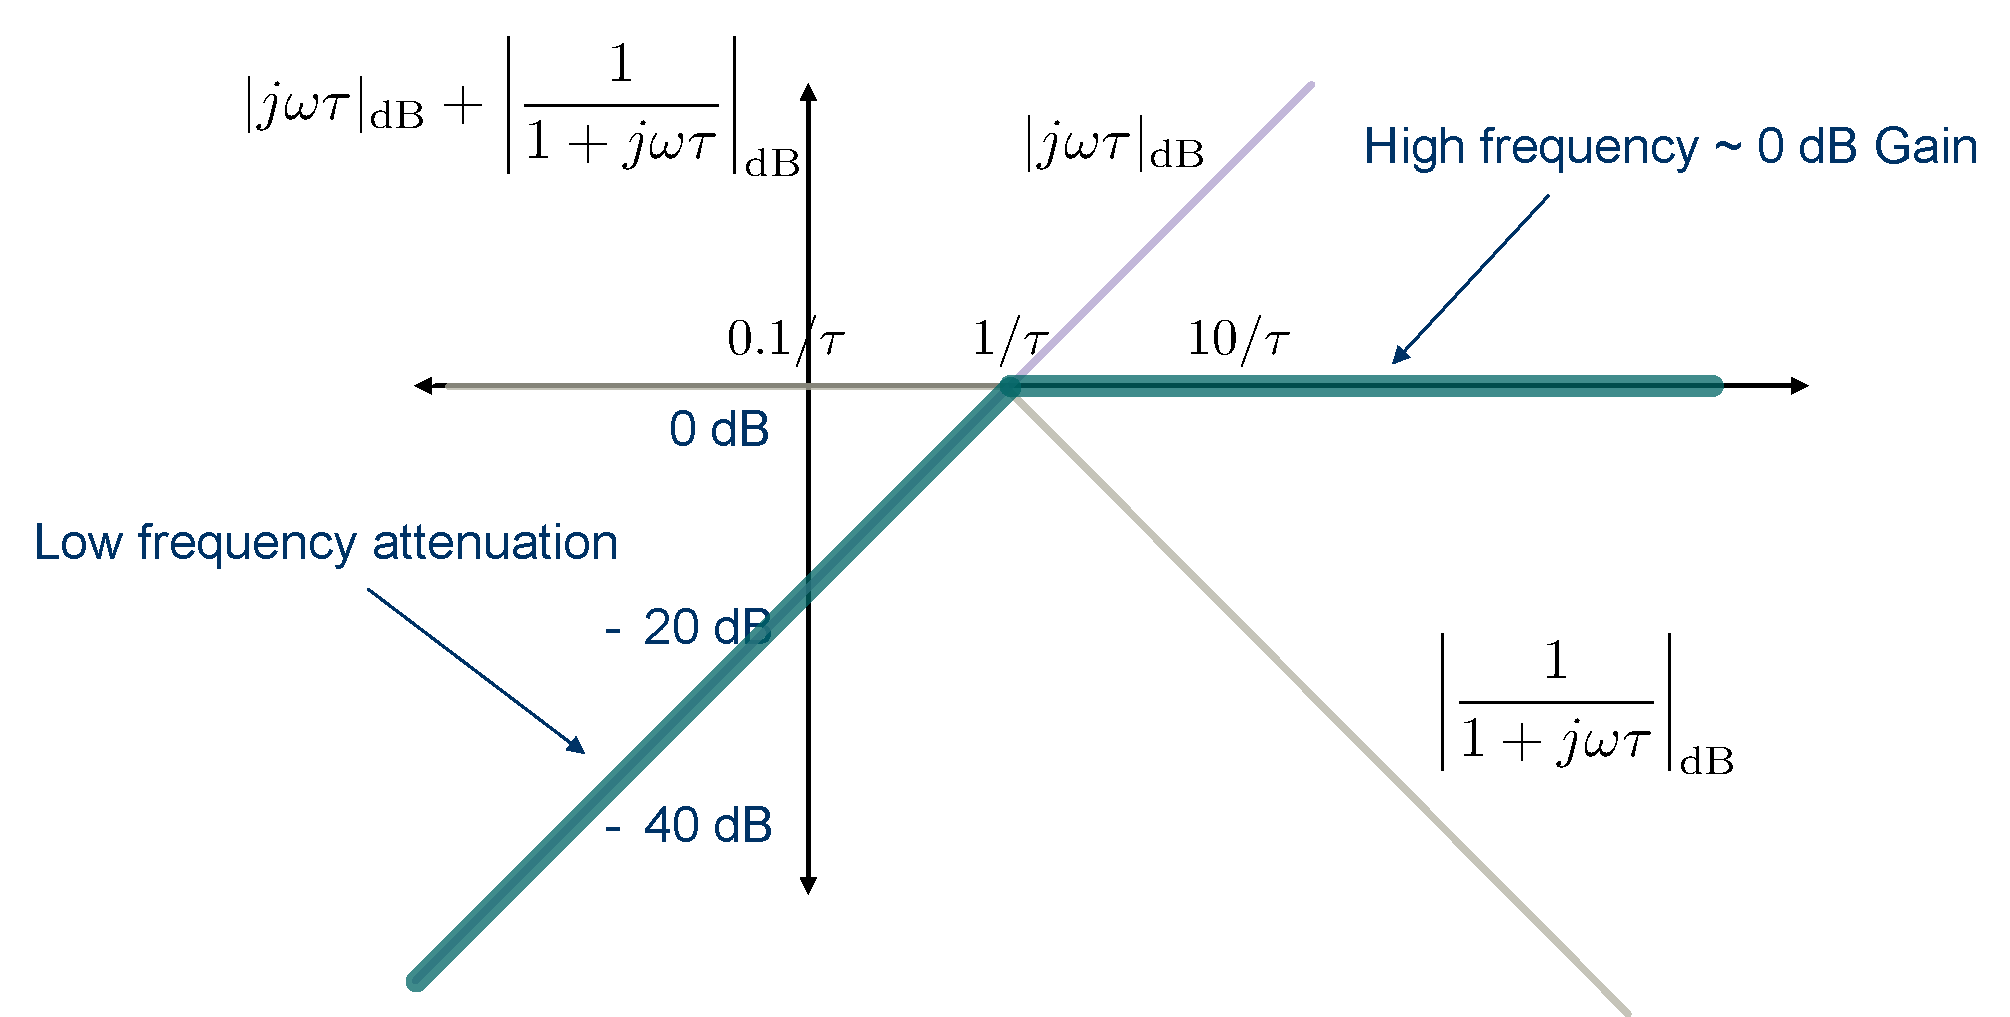
\includegraphics[width=.75\columnwidth]{mod1_3_11_bode3} \\
(a) \\
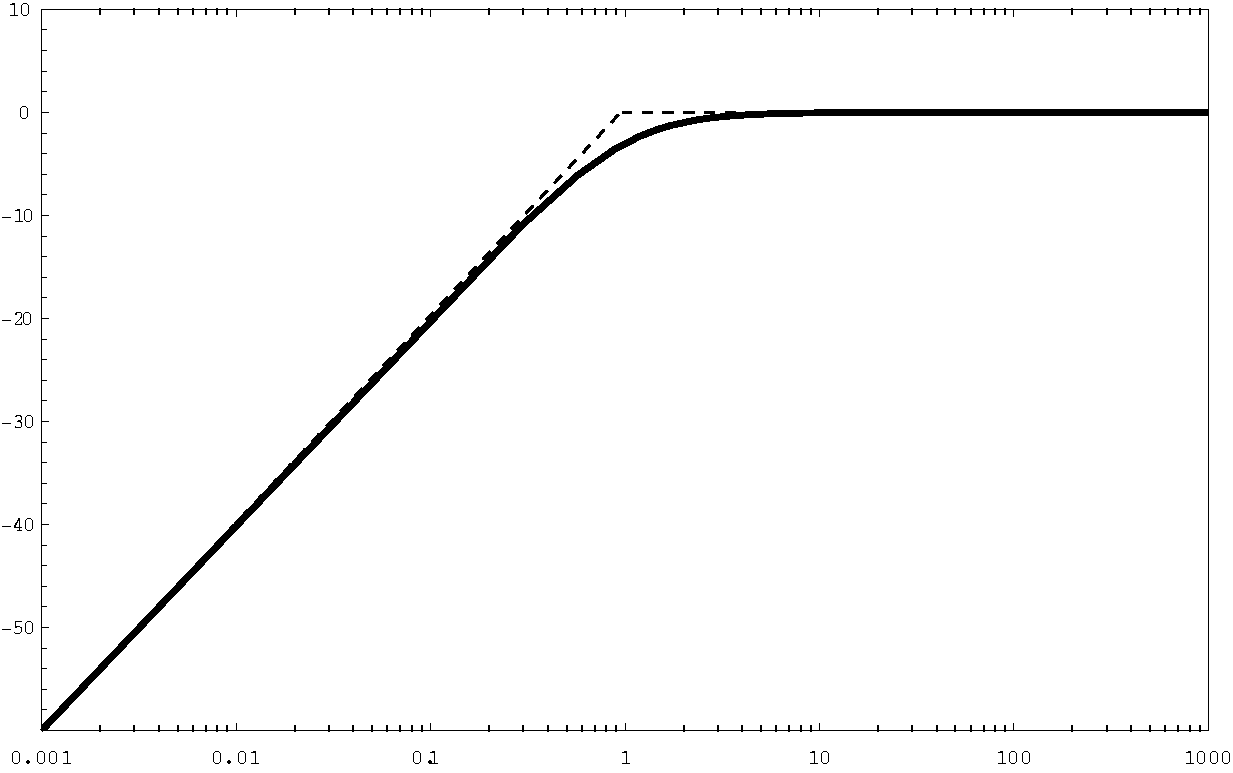
\includegraphics[angle=-0.0,width=.75\columnwidth]{mag_hpf} \\
(b) \\
\end{tabular}
\end{center}
\caption{(a) Composite Bode plot for the high-pass filter obtained by summing the shown component parts.  (b) A plot of the exact transfer function for the high-pass filter.} \label{fig:bode}
\end{figure}

For comparison, we also provide an overlay of the approximate curve and the actual plot (Fig.~\ref{fig:bode}b), and we see that the approximation is very accurate away from breakpoint.   At breakpoint there is a 3 dB error.



  
 


%%%%%%%%%%%%%%%%%%%%%%%%%%%%%%%%%%%%%%%%

\subsubsection{HPF Phase Plot}

Phase can be naturally decomposed as well:
\begin{equation} \angle H(\omega ) =  \angle \frac{{j\omega \tau }}{{1 + j\omega \tau }} =  \angle j\omega \tau  +  \angle \frac{1}{{1 + j\omega \tau }} = \frac{\pi }{2} - {\tan ^{ - 1}}\omega \tau \end{equation}
The first term is simply a constant phase of $90^\circ$ while the second term is the $\arctan$ function.  Estimate $\arctan$ function as shown using straight lines.  The rule of thumb is the line should break at a frequency of one tenth the breakpoint of the circuit, and end moving at a symmetrical point $10\times$ higher than the breakpoint.  See Fig.~\ref{fig:bode_phase}.
 
\begin{figure}[tb]
\begin{center}
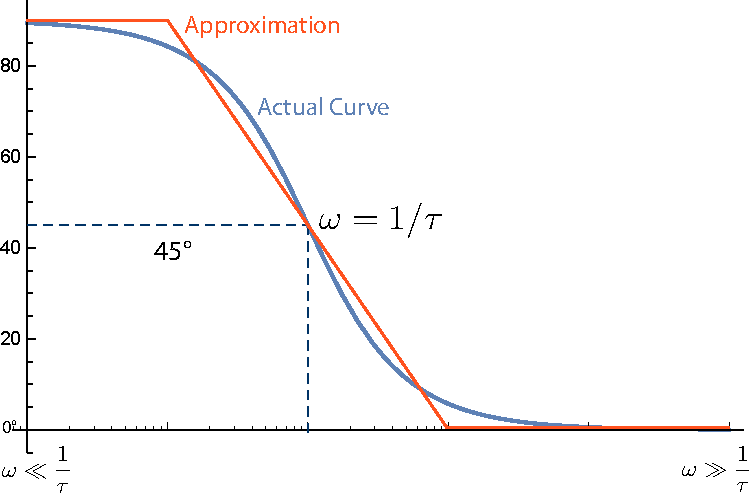
\includegraphics[width=.55\columnwidth]{mod1_3_12_bode4}
\end{center}
\caption{The approximate and exact phase response of the high-pass filter.} \label{fig:bode_phase}
\end{figure}


%\includegraphics[angle=-0.0,width=.75\columnwidth]{image_15.png}




%%%%%%%%%%%%%%%%%%%%%%%%%%%%%%%%%%%%%%%%
%%%%%%%%%%%%%%%%%%%%%%%%%%%%%%%%%%%%%%%%
%%%%%%%%%%%%%%%%%%%%%%%%%%%%%%%%%%%%%%%%

\section{Power Flow in AC Circuits}



%%%%%%%%%%%%%%%%%%%%%%%%%%%%%%%%%%%%%%%%
%%%%%%%%%%%%%%%%%%%%%%%%%%%%%%%%%%%%%%%%
%%%%%%%%%%%%%%%%%%%%%%%%%%%%%%%%%%%%%%%%





 The instantaneous power flow into any element is the product of the voltage and current: $P(t) = i(t)v(t)$.  For a periodic excitation, the average power is:
\begin{equation} 
{P_{av}} = \int\limits_T {i(\tau )v(\tau )d\tau } 
\end{equation}

In terms of sinusoids we have
 
{ \small
$\begin{array}{l}
{P_{av}} = \int\limits_T {\left| I \right|\cos (\omega t + {\varphi _i})\left| V \right|\cos (\omega t + {\varphi _v})d\tau } \\
 = \left| I \right| \cdot \left| V \right|\int\limits_T {(\cos \omega t\cos {\varphi _i} - \sin \omega t\sin {\varphi _i}} ) \cdot (\cos \omega t\cos {\varphi _v} - \sin \omega t\sin {\varphi _v})d\tau \\
 = \left| I \right| \cdot \left| V \right|\int\limits_T {d\tau {{\cos }^2}\omega t\cos {\varphi _i}\cos {\varphi _v} + {{\sin }^2}\omega t\sin {\varphi _i}\sin {\varphi _v} + c\sin \omega t\cos \omega t} \\
 = \frac{{\left| I \right| \cdot \left| V \right|}}{2}(\cos {\varphi _i}\cos {\varphi _v} + \sin {\varphi _i}\sin {\varphi _v}) = \frac{{\left| I \right| \cdot \left| V \right|}}{2}\cos ({\varphi _i} - {\varphi _v})
\end{array}$
}


%%%%%%%%%%%%%%%%%%%%%%%%%%%%%%%%%%%%%%%%

\subsection{Power Flow with Phasors}

The result of our calculation shows that the average power is simply given by
\begin{equation}
	{P_{av}} = \frac{{\left| I \right| \cdot \left| V \right|}}{2}\cos ({\varphi _i} - {\varphi _v})
\end{equation}
The phase term is sometimes denoted as the "power factor" and written as $PF$:
\begin{equation} 
	{P_{av}} = \frac{{\left| I \right| \cdot \left| V \right|}}{2} \cdot PF
\end{equation}
Note that if $({\varphi _i} - {\varphi _v}) = \frac{\pi }{2}$, then ${P_{av}} = \frac{{\left| I \right| \cdot \left| V \right|}}{2}\cos (\pi /2) = 0$.  This means that inductors and capacitors don't dissipate any energy.

An important lesson from this calculation is that since power is a non-linear function, we cannot simply take the real part of the product of the phasors:
\begin{equation}
	P \ne {\mathop{\rm Re}\nolimits} [I \cdot V]
\end{equation}
In fact, the correct answer can be deduced from our previous calculation:
\begin{equation}
	P = \frac{{\left| I \right| \cdot \left| V \right|}}{2}\cos ({\varphi _i} - {\varphi _v}) = \frac{1}{2}{\mathop{\rm Re}\nolimits} [I \cdot {V^*}] = \frac{1}{2}{\mathop{\rm Re}\nolimits} [{I^*} \cdot V]
\end{equation}

%%%%%%%%%%%%%%%%%%%%%%%%%%%%%%%%%%%%%%%%

\subsection{More Power to You!}

In terms of the circuit impedance we have:
\begin{equation}
\begin{array}{l}
	P = \frac{1}{2}{\mathop{\rm Re}\nolimits} [I \cdot {V^*}] = \frac{1}{2}{\mathop{\rm Re}\nolimits} [\frac{V}{Z} \cdot {V^*}] = \frac{{{{\left| V \right|}^2}}}{2}{\mathop{\rm Re}\nolimits} [{Z^{ - 1}}]\\
   = \frac{{{{\left| V \right|}^2}}}{2}{\mathop{\rm Re}\nolimits} [\frac{{{Z^*}}}{{{{\left| Z \right|}^2}}}] = \frac{{{{\left| V \right|}^2}}}{{2{{\left| Z \right|}^2}}}{\mathop{\rm Re}\nolimits} [{Z^*}] = \frac{{{{\left| V \right|}^2}}}{{2{{\left| Z \right|}^2}}}{\mathop{\rm Re}\nolimits} [Z]
\end{array}
\end{equation}
Check the result for a real impedance (resistor) to verify we have not made any errors.   Also, in terms of current:
\begin{equation}
	P = \frac{1}{2}{\mathop{\rm Re}\nolimits} [{I^*} \cdot V] = \frac{1}{2}{\mathop{\rm Re}\nolimits} [{I^*} \cdot I \cdot Z] = \frac{{{{\left| I \right|}^2}}}{2}{\mathop{\rm Re}\nolimits} [Z]
\end{equation}

 



%%%%%%%%%%%%%%%%%%%%%%%%%%%%%%%%%%%%%%%%

\subsection{Understanding AC Power Flow}


\begin{figure}[tb]
\begin{center}
\begin{tabular}{cc}
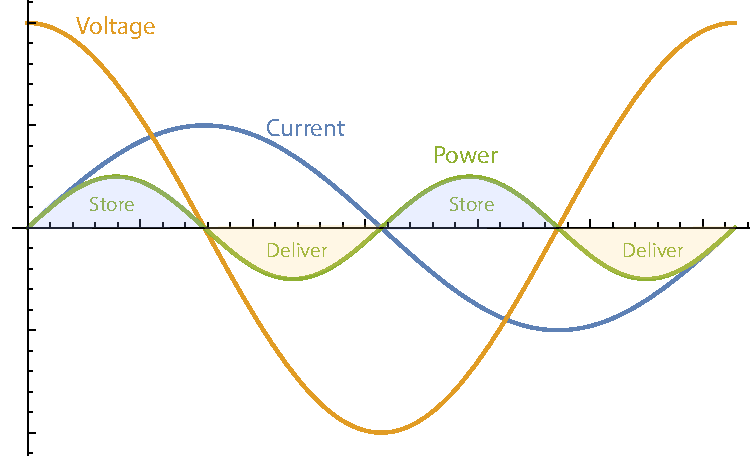
\includegraphics[width=.5\columnwidth]{cap_power} &
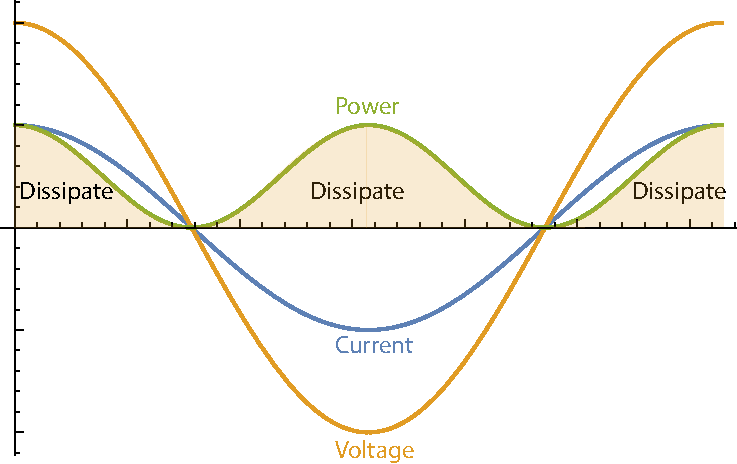
\includegraphics[width=.5\columnwidth]{res_power} \\
(a) & (b) \\
\end{tabular}
\end{center}
\caption{(a) The current and voltage waveforms in a reactive circuit are $90^\circ$ out of phase whereas (b) for a resistive circuit, they are in phase.} \label{fig:powerflow}
\end{figure}

Notice that if the voltage and the current are $90^\circ$ out of phase (inductors and capacitors), then their product is such that during one half the cycle power flows in, and in the other half cycle power flows out, as illustrated in Fig.~\ref{fig:powerflow}.  This means there's no net power flow into these components.  For a resistor, on the other hand, since current and voltage are in phase, it doesn't matter what direction current flows, it's always in phase with the voltage and dissipating power.  Also, power flows twice per cycle!


%%%%%%%%%%%%%%%%%%%%%%%%%%%%%%%%%%%%%%%%

\subsection{Chapter Summary}

In this chapter we demonstrated that phasor analysis allows us to treat all $LCR$ circuits as simple “resistive” circuits by using the concept of impedance (admittance).  While the frequency response allows us to completely characterize a system, we also showed that we can also characterize the system by the locations of its poles and zeros.  The Bode plot is a very useful tool for sketching the transfer function in the $\log$-$\log$ domain once we know the location of the poles and zeros.  Ultimately, we'll learn that the location of poles/zeros is the key to understanding how a linear system will respond to inputs or even initial conditions (charges on capacitors, currents in inductors).
 
 



